%%
%% This is file `mcmthesis-demo.tex',
%% generated with the docstrip utility.
%%
%% The original source files were:
%%
%% mcmthesis.dtx  (with options: `demo')
%% 
%% -----------------------------------
%% 
%% This is a generated file.
%% 
%% Copyright (C)
%%     2010 -- 2015 by Zhaoli Wang
%%     2014 -- 2016 by Liam Huang
%% 
%% This work may be distributed and/or modified under the
%% conditions of the LaTeX Project Public License, either version 1.3
%% of this license or (at your option) any later version.
%% The latest version of this license is in
%%   http://www.latex-project.org/lppl.txt
%% and version 1.3 or later is part of all distributions of LaTeX
%% version 2005/12/01 or later.
%% 
%% This work has the LPPL maintenance status `maintained'.
%% 
%% The Current Maintainer of this work is Liam Huang.
%% 
\documentclass{mcmthesis}
\mcmsetup{CTeX = false,   % 使用 CTeX 套装时,设置为 true
        tcn = 2020042, problem = C,
        sheet = true, titleinsheet = true, keywordsinsheet = true,
        titlepage = false, abstract = true}
\usepackage{palatino}
\usepackage{lipsum}
\usepackage{indentfirst}
\usepackage{booktabs}
\usepackage{graphicx}
\usepackage{enumitem}
\usepackage[section]{placeins} % 禁止图表跨过section
\setlength{\parindent}{2em}
\setlength{\parindent}{2em}


\title{Commercial Opportunities beneath Reviews}
\author{\small \href{http://www.latexstudio.net/}
  {
\includegraphics[width=7cm]{mcmthesis-logo}}}
\date{\today}
\begin{document}
\begin{abstract}

  In order to choose the most appropriate online sales strategy and find potentially important design features, our team makes an analysis on the data and find the hidden relationship between several measures, especially based on time. We completed the following works to provide Sunshine Company a comprehensive profile to make business decisions.

Firstly, we preprocess the data, including missing value imputation, data cleaning, abnormal characters transformation. Based on our dataset partition and review separation, we separately use Naïve Bayes Classifier and LSTM to achieve the sentiment analysis, which provide us a relatively objective sentiment evaluation based on reviews.

Next, we construct the AHP-FCE model to reflect the reputation of product in a period of time. We classify different indicators and divide them into three levels. By using FCE model, we obtain a preliminary evaluation of products’ reputation. 

Moreover, we further propose the Multivariate Nonlinear Regression Model based on market factors. We target the number of reviews and construct a function related with several factors, based on the assumption that the number of reviews is positively correlated with the purchase. 

We consider the potential influence of history reviews on future reviews and use the simplified time series. In order to fit the data better, we also introduce the number of effective fans and the occurrence of market events to the model and obtain the relationship between several factors. 

According to this, we can provide a more appropriate online sales strategy for the company.


Finally, we analyze potentially important features of specific products, and find the most influential “words” to evaluate the quality of a product.


\begin{keywords}
Sentiment Analysis; Market Factor
\end{keywords}
\end{abstract}

\maketitle


\tableofcontents

\newpage

\section{Introduction}

\subsection{Problem Restatement}

With the rapid development of technology and logistics, there is an increasing number of people choosing shopping online. While the customers open the parcel and enjoy the shopping, the sellers receive feedbacks based on their “reviews” and “star ratings”, which express the customers’ level of satisfaction. Moreover, other customers can also submit ratings on these reviews as being helpful or not.

Firstly, we programmed data processing and made a comprehensive analysis on the patterns of reviews. After that, we obtained a relatively objective rating of sentiment based on the reviews.

Secondly, we synthesized several elements, including sentiment, star ratings, proportion of helpful votes, and constructed the “reputation point” to reflect public’s synthetic preference of specific products.

Finally, based on the “reputation point” we gave, we analyzed the hidden relationship between people’s expectation, the potential of specific products, and time. 




\section{Assumption}

\begin{enumerate}
  \item \textbf{Balance Supply and Demand Hypothesis}\\
  We assumed that supply and demand on American market are balanced on the whole. 
  \item \textbf{Consumer Preference Hypothesis} \\
  Consumer Preference Hypothesis. Consumer preference of a specific product does not change in a period of time.
  \item \textbf{Authentic Data Hypothesis} \\
  We assume all the data provided is authentic and original. 
\end{enumerate}

\section{Data Preprocessing}

\begin{enumerate}
  \item Select the target products. We only need to focus on hair dryer, pacifier and microwave, but the data provided includes several products other than our targets, for example, infant care kit. So we first selected our target products from the data set.
  \item Transform the abnormal characters. We find there are many abnormal characters in the data set. Emoji, foreign language and HTML tags will have a negative impact on further data programming. We used appropriate regular expressions to filter and translate some of them.
  \item Missing value interpolation. Some of the reviews’ contents are missing. If this kind of reviews have a title, we use the title to replace its contents, otherwise we removed this review from the data set.
  \item Data nationality test. We checked the nationality of the data. For example, if the number of helpful votes is smaller than that of total votes.
\end{enumerate}


\section{Sentiment Analysis}

We use two methods to do our sentiment analysis: Naive Bayes Classifier 
and LSTM. Both have their advantages and disadvantages.

The advantage of Naive Bayes Classifier is that it can extract features from the text, which enables us to do a wordcloud. The disadvantage of Naive Bayes Classifier is that it doesn't consider the relationship of words, which is so-called context. 


The advantage of LSTM is that it consider the relationship of words, which leads to a better accuracy. The disadvantage of LSTM is that it is an uninterpretable blackbox, which is a common defect of neural networks.


\subsection{Dataset Partition}

We select out reviews that are rated one star and five stars as our train-test set, where reviews with one star are tagged as "pos" and reviews with five stars are tagged as "neg". We use $70\%$ of the train-test set as our train set and use remaining $30\%$ as our test set.

We train models respectively for hair dryer, pacifier and microwave. The test accuracy are all above $0.90$


\subsection{Naive Bayes Classifier}


Naive bayes classifier is a probabilistic classifiers 
based on applying Bayes' theorem with strong independence assumptions between the features.

We use the Naive Bayes Classifier from TextBlob. We have extracted featrues from both postive reviews and negative reviews. Below are what we found in these reviews.

Fig.\ref{fig:hair_dryer_pos_wordcloud} and Fig.\ref{fig:hair_dryer_neg_wordcloud} are the wordclouds based on the featrues of postive reviews and negative reviews of hair dryers. We can note that in the negative wordcloud, the words "spark", "dangerous", "fire" appear frequently, which indicates that the company needs to pay more attention to safety issues if it wants to make an achievement in the hair dryer's market. 

\begin{figure}[!h]
\centering
\begin{minipage}[t]{0.48\textwidth}
\centering
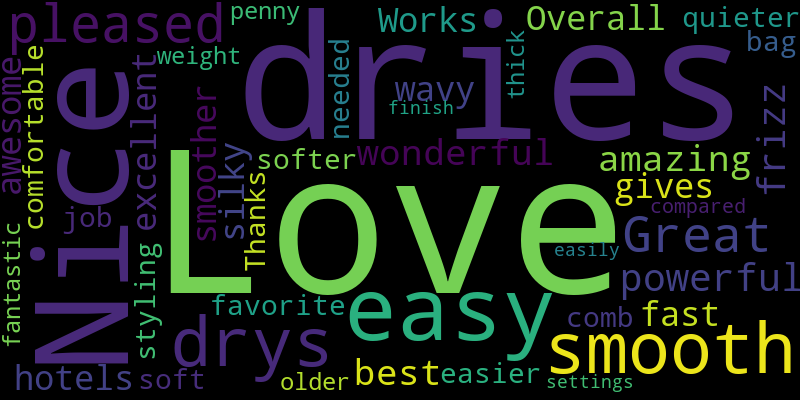
\includegraphics[width=6cm]{hair_dryer_pos_wordcloud.png}
\caption{Hair dryer postive wordcloud}
\label{fig:hair_dryer_pos_wordcloud}
\end{minipage}
\begin{minipage}[t]{0.48\textwidth}
\centering
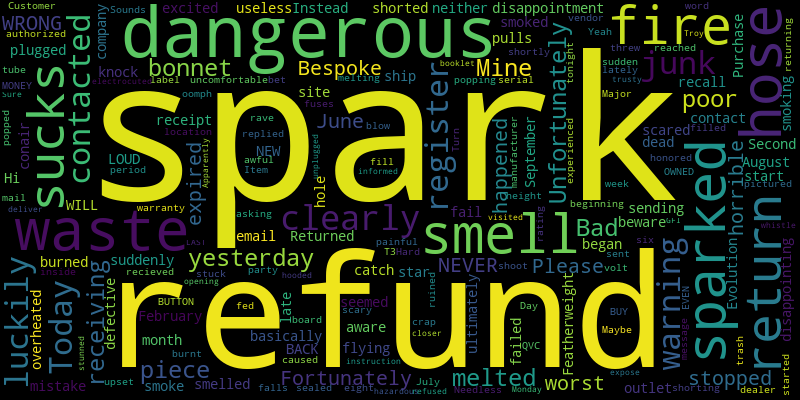
\includegraphics[width=6cm]{hair_dryer_neg_wordcloud.png}
\caption{Hair dryer negative wordcloud}
\label{fig:hair_dryer_neg_wordcloud}
\end{minipage}
\end{figure}



Fig.\ref{fig:pacifier_pos_wordcloud} and Fig.\ref{fig:pacifier_neg_wordcloud} are the wordclouds based on the featrues of postive reviews and negative reviews of pacifiers. As we can note, "cute" is cited a lot in the postive reviews. Hence a pacifier which is cute and lovely may attract babies' attention.

\begin{figure}[!h]
\centering
\begin{minipage}[t]{0.48\textwidth}
\centering
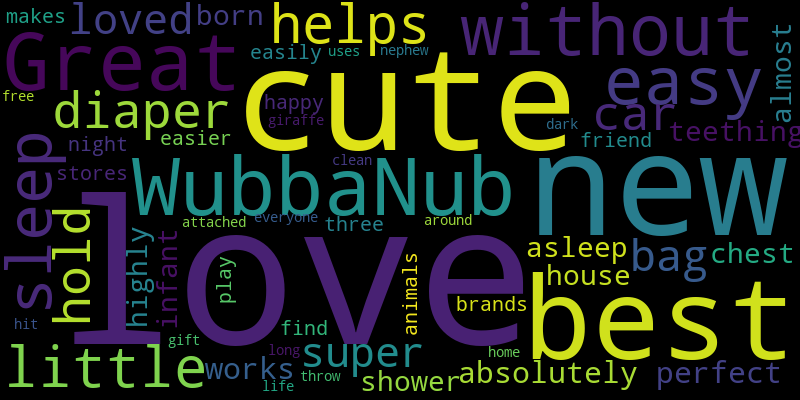
\includegraphics[width=6cm]{pacifier_pos_wordcloud.png}
\caption{Pacifier postive wordcloud}
\label{fig:pacifier_pos_wordcloud}
\end{minipage}
\begin{minipage}[t]{0.48\textwidth}
\centering
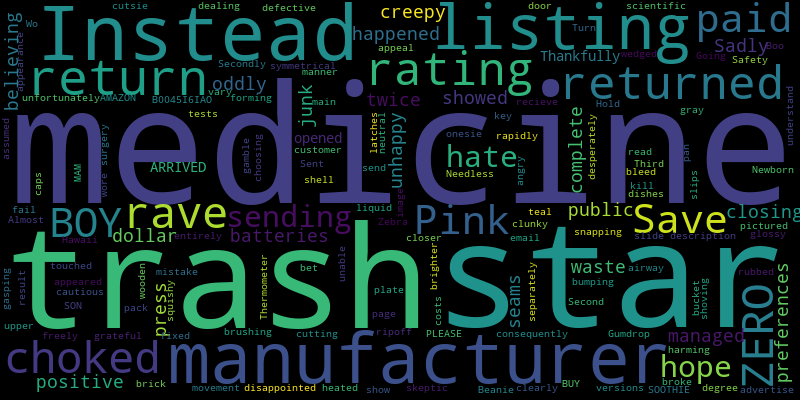
\includegraphics[width=6cm]{pacifier_neg_wordcloud.png}
\caption{Pacifier negative wordcloud}
\label{fig:pacifier_neg_wordcloud}
\end{minipage}
\end{figure}



Fig.\ref{fig:microwave_pos_wordcloud} and Fig.\ref{fig:microwave_neg_wordcloud} are the wordclouds based on the featrues of postive reviews and negative reviews of microwaves. In the negative wordcloud of microwave, "repair" and "warranty" stand out, which reveals that consumers mostly complain about the malfunction of the machines and unsatisfactory warranty. Companies that want make a success in microwave market should consider better after-sale service. Also they need to improve their products' quality.

\begin{figure}[!h]
\centering
\begin{minipage}[t]{0.48\textwidth}
\centering
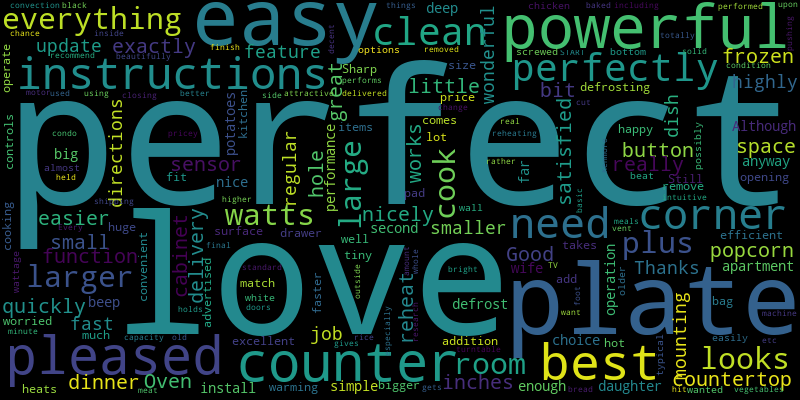
\includegraphics[width=6cm]{microwave_pos_wordcloud.png}
\caption{Microwave postive wordcloud}
\label{fig:microwave_pos_wordcloud}
\end{minipage}
\begin{minipage}[t]{0.48\textwidth}
\centering
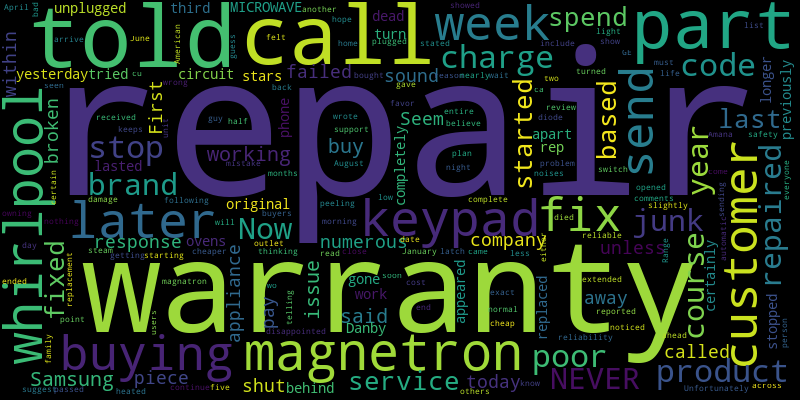
\includegraphics[width=6cm]{microwave_neg_wordcloud.png}
\caption{Microwave negative wordcloud}
\label{fig:microwave_neg_wordcloud}
\end{minipage}
\end{figure}





\subsection{LSTM}

LSTM is so-called long short-term memory. It is a kind of recurrent neural network(RNN). It differs from standard feedforward neural networks in that it has feedback connections. It is built for sequences of data instead of single data points, which makes it a good choice to do sentiment analysis since reviews also have contexts. We need these contexts to better predict the sentiment based on the text.

Our model structure is revealed as Fig.\ref{fig:model}. And the LSTM's structure is revealed as Fig.\ref{fig:lstm}



\begin{figure}[!h]
  \small
  \centering
  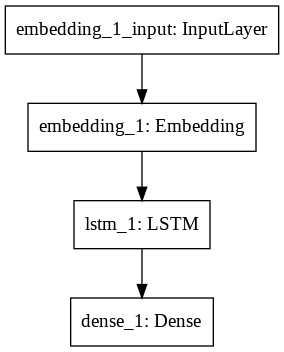
\includegraphics[width=4cm]{model.png}
  \caption{Model structure} \label{fig:model}
\end{figure}


\begin{figure}[!h]
  \small
  \centering
  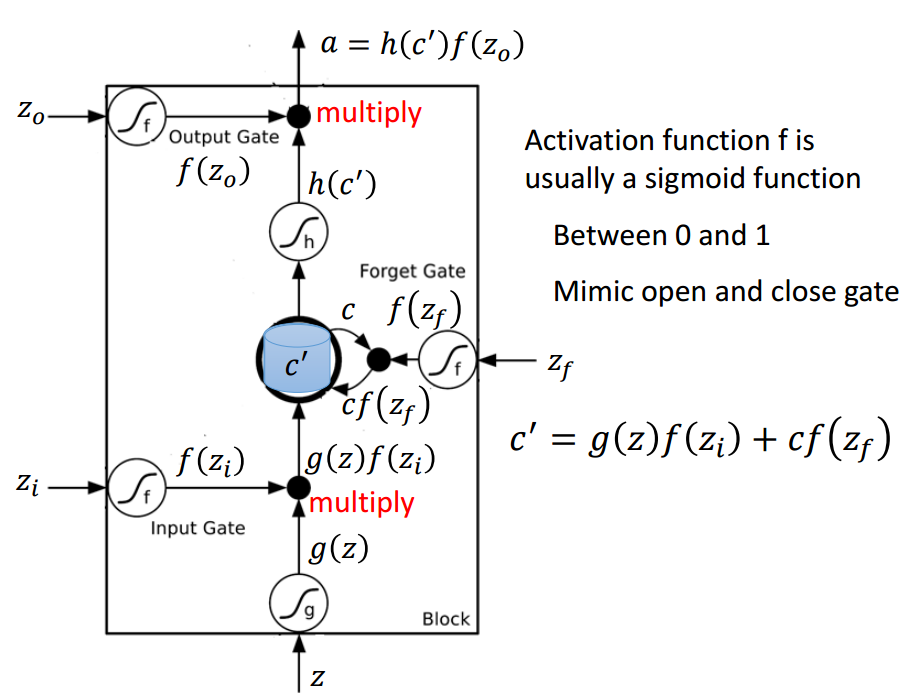
\includegraphics[width=8cm]{lstm.png}
  \caption{LSTM structure} \label{fig:lstm}
\end{figure}


Some predicted results are showed in Table.\ref{tab:result}

\begin{table}[!h]
  \centering
  \caption{Some predicted results of LSTM} 
  \label{tab:result}
  \begin{tabular}{ll}
  \toprule[2.5pt]
  \textbf{Reviews}& \textbf{Results} \\
  \midrule[1.5pt]
  i really like this hairdryer  & \\ 
  i havent had it very long   &  0.9990048 \\
  but its working well for me  &  \\
  \midrule 
  was a great dryer loved it  & 0.06360153 \\
  however it burned out within 2 months &  \\
  \midrule 
  clumsy apparatis i wanted more mobility  like multitacking & \\ 
  and this is not set up to run with the flow &  0.5436161\\
   hose waned to stay on box and i wanted it to travel with me & \\
    my own problem  it was meant to be stable & \\

  \bottomrule
  \end{tabular}
  \end{table}



\section{AHP-FCE model}

We used AHP-FCEM (Analytic Hierarchy Process-Fuzzy comprehensive evaluation model) to synthesize and conclude the characteristic of customers’ opinions.

Firstly, we conducted Correlation Test of several elements provided. According to the scatterplot and the correlation matrix, we found a strong linear correlation between the number of helpful votes and that of total votes, which is coordinated with common sense. Therefore, we combined this two elements into “the proportion of helpful votes” for further use. 

Meanwhile, in order to reflect the representativeness of data, we calculated every week’s average value of each element. 

Moreover, we also transformed “N” into 0 and “Y” into 1 to express the value of “vine“ and “verified purchase”. We set three levels to evaluate the degree of “verified purchase” and two levels to evaluate that of “vine”. 

\begin{table}[!h]
  \centering
  \caption{Main Symbols used in AHP-FCE repution Model} %\label{tab:aStrangeTable}
  \begin{tabular}{ll}
  \toprule[2.5pt]
  \textbf{Symbols}& \textbf{Definition} \\
  \midrule[1.5pt]
   $TR_t$ & Total reviews in week $t$ \\
   \midrule 
   $TV_t$ & Total votes in week $t$ \\
   \midrule 
   $APH_t$ & Average proportion of helpful votes in week $t$ \\
    \midrule 
    $ASP_t$ & Average sentiment point in week $t$ \\
    \midrule 
    $ASR_t$ & Average star ratings in week $t$ \\
    \midrule 
    $AV_t$ & Average number of vine in week $t$ \\ 
    \midrule 
    $AVP_t$ & Average number of verified purchase in week $t$ \\
  \bottomrule
  \end{tabular}
  \end{table}


  \begin{figure}[!h]
    \small
    \centering
    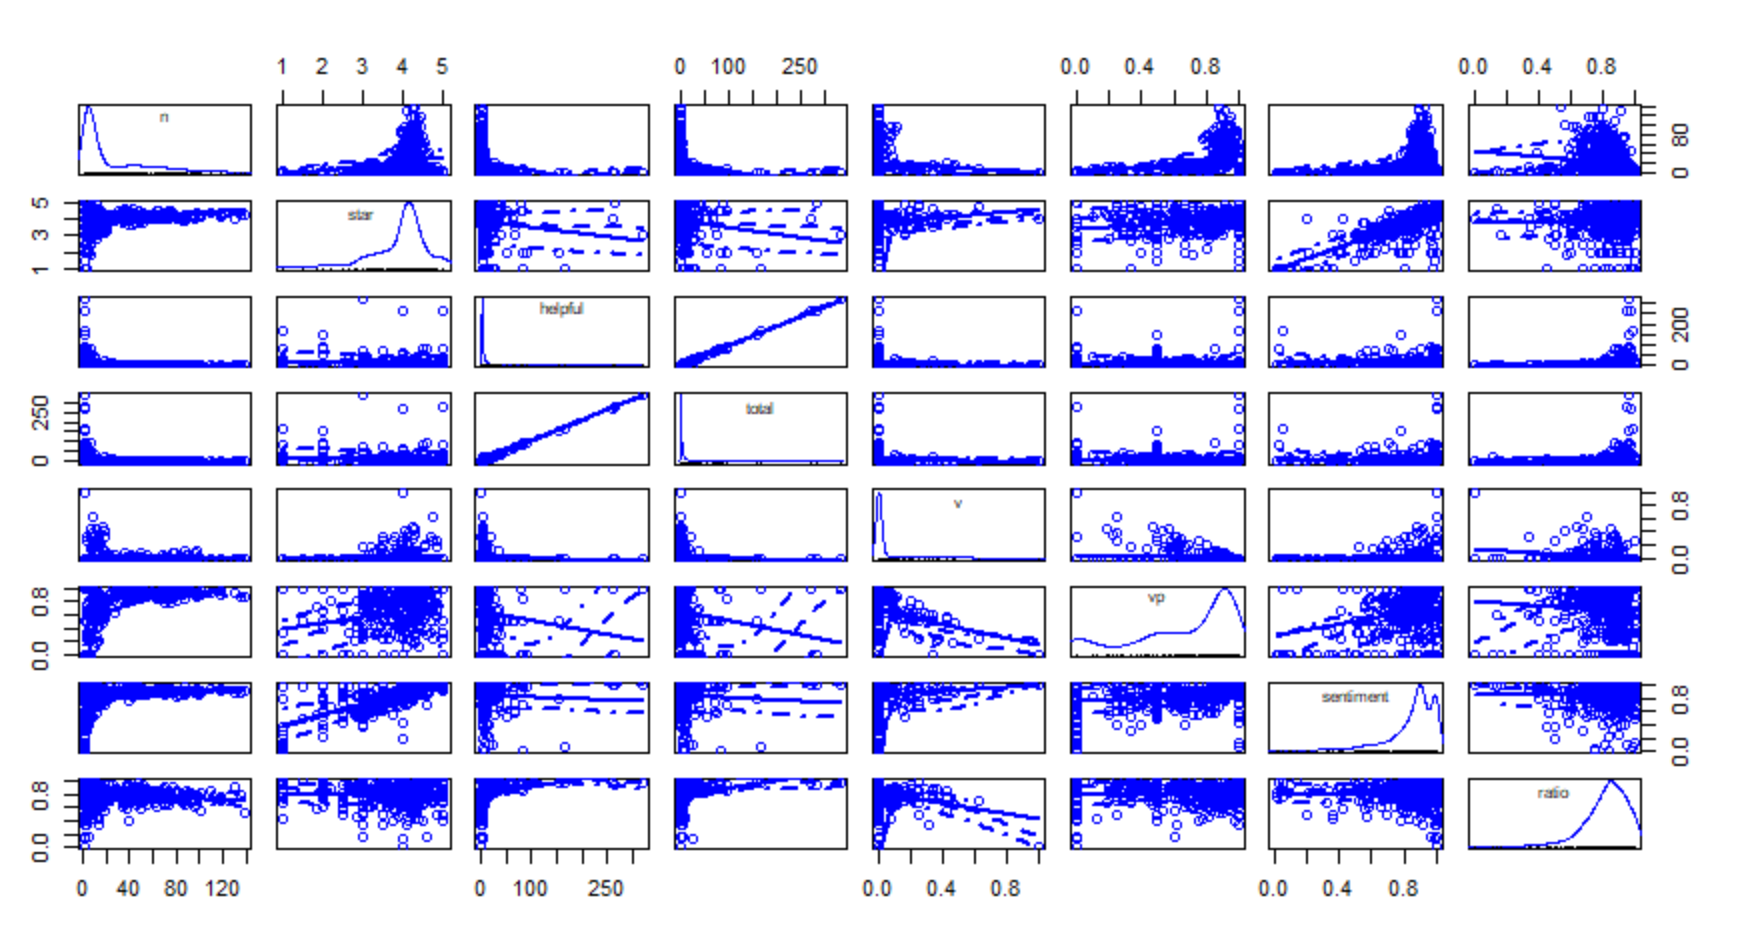
\includegraphics[width=8cm]{relative_matrix.png}
    \caption{Correlation matrix} %\label{fig:lstm}
  \end{figure}

  \begin{equation}
    VL = \begin{cases}
      2, & \text{if } AV_t \ge 0.05 \\
      1, & \text{if } AV_t < 0.05
    \end{cases}
  \end{equation}

  \begin{equation}
    VPL = \begin{cases}
      3, & \text{if } AVP_t \in (0.8, 1] \\
      2, & \text{if } AVP_t \in (0.5, 0.8] \\
      1, & \text{if } AVP_t \in  [0, 0.5] 
    \end{cases}
  \end{equation}


  According to the elements provided in the data set, we conducted the following classification. The number of total reviews and number of total votes reflect the popularity of a product in a week. The satisfaction degree is combined with the proportion of helpful votes, review’s sentiment points and the star ratings customers gave. We also measured if a review is convincing by using the average number of vine and that of verified purchase.

  \begin{figure}[!h]
    \small
    \centering
    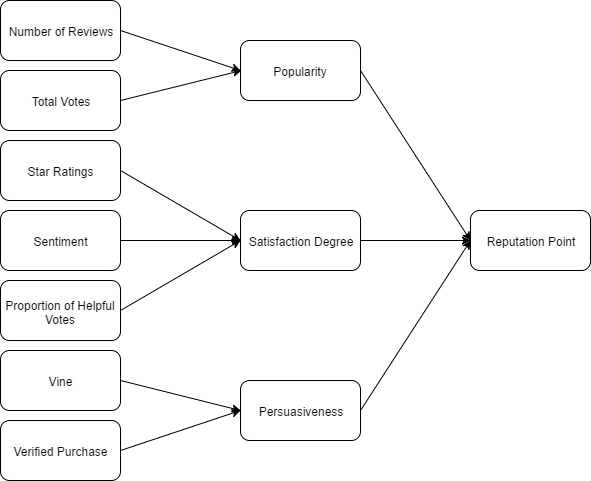
\includegraphics[width=8cm]{classifier.jpg}
    \caption{Classifier} %\label{fig:lstm}
  \end{figure}


  \begin{equation}
    \begin{aligned}
      \text{popularity}: & POP_t  = \frac{1}{6} \log{(10 TR_t)} \cdot \log{(TV_t + 10)} \\
      \text{Perservasiveness}: & PER_t = VL \cdot VPL \\
      \text{Satisfaction Degree}: & SD_t = \frac{1}{45} APH_t \cdot ASP_t \cdot ASR_t
    \end{aligned}
  \end{equation}

  Based on this, we made the following FCEM model.  $R_t$ represents the common reputation of specific product in a week.

  \begin{equation}
    R_t = PER_t (0.4 POP_t + 0.6 PER_t)
  \end{equation}


  \begin{figure}[!h]
    \small
    \centering
    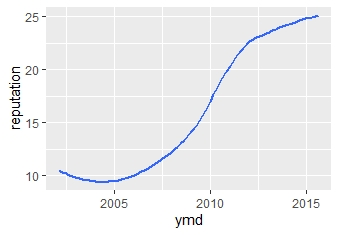
\includegraphics[width=8cm]{ymd_reputation2.jpeg}
    \caption{Reputation to time 2002-2015} %\label{fig:lstm}
  \end{figure}


\section{Multivariate nonlinear regression model based on simplified time series}


\begin{table}[!h]
  \centering
  \caption{Main Symbols used in MLR Model} %\label{tab:aStrangeTable}
  \begin{tabular}{ll}
  \toprule[2.5pt]
  \textbf{Symbols}& \textbf{Definition} \\
  \midrule[1.5pt]
   $a$ &  parameters  \\
   \midrule
   $b$ & parameters \\
   \midrule
   $c$ & parameters \\
   \midrule
   $msr_t$ & The mean of star rating at time $t$ \\
   \midrule
   $ms_t$ & The mean of sentiment at time $t$ \\
   \midrule
   $mr_t$ & The mean of ratio at time $t$ \\
   \midrule 
   $\alpha$ & The percentage of buyers willing to comment \\
   \midrule 
   $\beta$ & Scope of information dissemination \\
   \midrule 
   $\gamma$ &  The rate of decline in the proportion of information \\
    \midrule
    $R1_t$ & Proportion of information recipients converted to buyers at time $t$ \\
    \midrule 
    $R2_t$ & The amount of information propagated at time $t$ \\
    \midrule 
    $Irp_t$ & The downward pressure on the proportion of information at time $t$  \\
    \midrule  
    $pb_t$ &  Effective number of fans at time $t$  \\
    \midrule 
    $mrp_t$ & The pressure of the total market expansion \\
    & leads to a decline in market influence at time $t$ \\
    \midrule 
    $ss_t$ & Simplified random event effects at time $t$ \\
  \bottomrule
  \end{tabular}
  \end{table}


Parameter description:

\begin{equation}
  \begin{aligned}
    Reputation & = \alpha * R1_t * R2_t * Irp_t + pb_t + mrp_t *ss_t \\
    \alpha &= 0.9 \\
    \beta & = 1.4 \\
    \gamma & = -0.01 \\
    R1_t &= a*msr_t + b*ms_t + c*mr_t \\
    R2_t & = \exp{(\beta * t^{\frac{1}{4}})} \\
    Irp_t & = \exp{(\gamma * t^{\frac{1}{2}})} \\
    pb_t & = 1 / (a*msr_t + b*ms_t + c* mr_t) \\
    mrp_t &= \exp{(-t^{\frac{1}{8}})} \\
    ss_t &= (-t^{\frac{1}{4}})^3 \\
  \end{aligned}
\end{equation}




Explanation:

Under the assumption that the number of reviews is positively correlated with the purchase.

Amount, we believe that the reputation of a product will be affected by the following quantities: the number of reviews, the number of effective fans and the occurrence of market events.

\begin{itemize}
  \item The number of reviews: \\
  \begin{enumerate}
    \item With the help of the Internet, the spread of commodity information will increase exponentially with time, that is, $R2_t$.
    \item However, as the amount of information in the whole Internet increases over time, the information proportion of this commodity decreases exponentially, and the rate of decline is measured by $\gamma$, $Irp_t$ represents the impact of the decline((the percentage of product information that can be seen by people)。The true number of information receivers at time t is: $R2_t * Irp_t$. 
    \item $R1_t$ is not only the ratio of information receiver to buyer, but also the influence degree of comment emotion
  \end{enumerate}
  So the number of comments is equal to $\alpha * R1_t * R2_t * Irp_t$

  \item The number of effective fans: \\
    \begin{enumerate}
      \item We divided the fans of merchandise into two categories: effective fans and invisible fans, Effective fans will help the sales and reputation of the products by increasing the purchase volume and scanning comments. Due to a series of difficulties, invisible fans will not take action in normal times, and only when the product is impacted, they will buy it. The number of effective fans means the number of potential purchases. 
      \item When the comment sentiment level $R1_t$ is relatively low, it indicates that the product is hit by negative comments. At this time, fans will maintain the image of the product by increasing the amount of purchase and comments.Therefore, the reduction of $R1_t$ can promote the increase of effective fans
    \end{enumerate}
  \item The occurrence of market events: \\
  \begin{enumerate}
    \item We assume that the market attention of a commodity is positively related to its age in the market. At the same time, positive and negative events occur randomly. To simplify the random factor, we alternate positive and negative events. The combination of event nature and market attention of the commodity constitutes $ss_t$, which will affect the reputation of the commodity.
  \end{enumerate}

\end{itemize}

Through multiple nonlinear regression, We take $\alpha$=0.9, $\beta$=1.4, $\gamma$=-0.01, $a$=0.2, $b$=0.5, $c$=0.3, and obtained Fig.\ref{fig:bc2}:


\begin{figure}[!h]
  \small
  \centering
  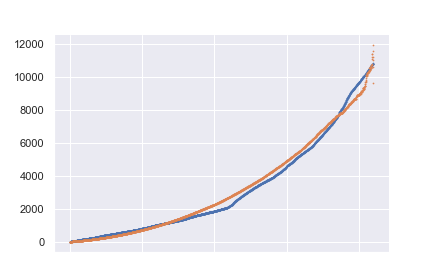
\includegraphics[width=10cm]{bc2.png}
  \caption{Simulation Curve of Reputation} \label{fig:bc2}
\end{figure}



Among them, the blue curve is the total market sales volume (cumulative volume), and the yellow curve is reputation.
As can be seen, reputation better reflects the changing trend of total market sales. Due to the mathematical definition of reputation, it is bounded. At the same time, as t approaches infinity, reputation will approach zero. These two properties indicate that the influence of goods is limited and it will be eliminated from the market over time, which is consistent with our common sense.




\section{Correlation Test}

In terms of individual products, the number of stars in year n will affect the number of reviews in year n+1, and this influence will gradually increase.

From 2008 to 2015, the average star number of each product in the previous year and the total number of reviews in the following year were calculated, and the following distribution relationship was obtained. It can be seen that from 2008 to 2013, the impact of different star rating on the number of reviews in the next year is gradually obvious. Compared with low star rating, products with high star rating are more likely to receive more reviews in the second year. In 2014 and 2015, the average star rating of most products was between 3 and 5, and there was still a positive correlation between star rating and the number of reviews.

\begin{figure}[!h]
  \small
  \centering
  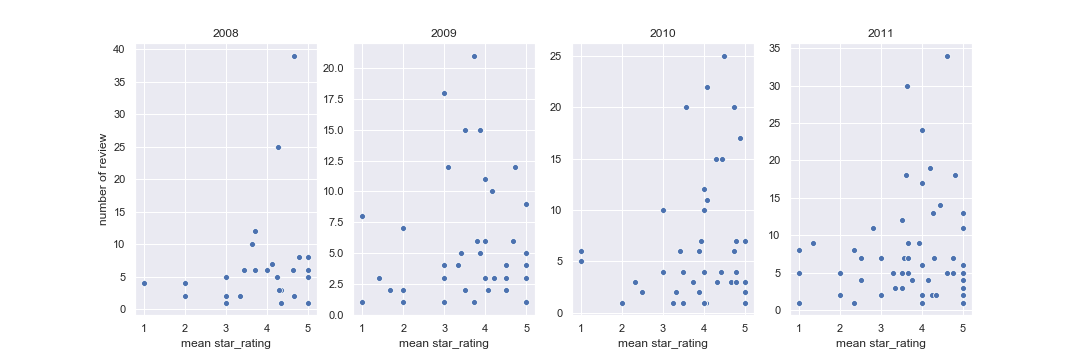
\includegraphics[width=10cm]{mean_star_rating_to_number_of_review_2008-2011.png}
  \caption{Mean star rating to number of review 2008-2011} %\label{fig:lstm}
\end{figure}

\begin{figure}[!h]
  \small
  \centering
  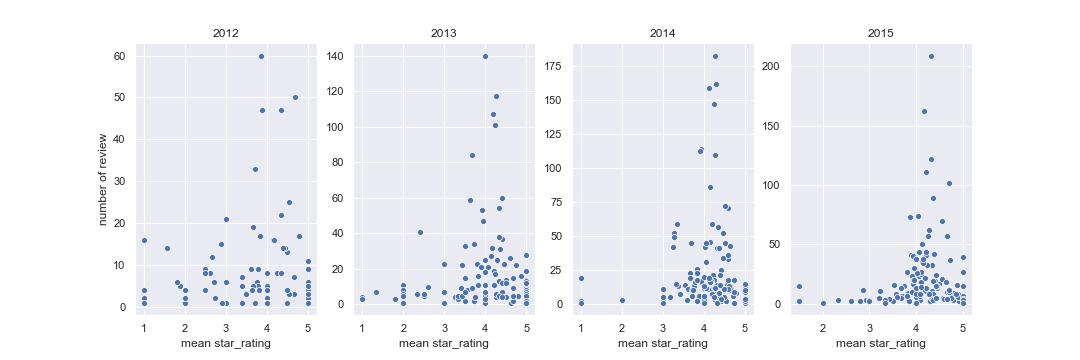
\includegraphics[width=10cm]{mean_star_rating_to_number_of_review_2012-2015.png}
  \caption{Mean star rating to number of review 2012-2015} %\label{fig:lstm}
\end{figure}

In terms of the whole market, the distribution relationship between stars and comments is relatively stable. 1,2 stars will bring less comments, while 4,5 stars will bring more comments.

In each year, the number of stars and comments conforms to the quadratic relation, and satisfies: the number of comments in the second year corresponding to 1 and 2 stars is relatively low, while the number of comments in the second year corresponding to 4 and 5 stars is relatively high.After observing the data set, it is found that since most consumers have distinct emotions, the polarization degree of starmaking is high, so the number of comments in the middle of three stars is lower than that in the low stars

\begin{figure}[!h]
  \small
  \centering
  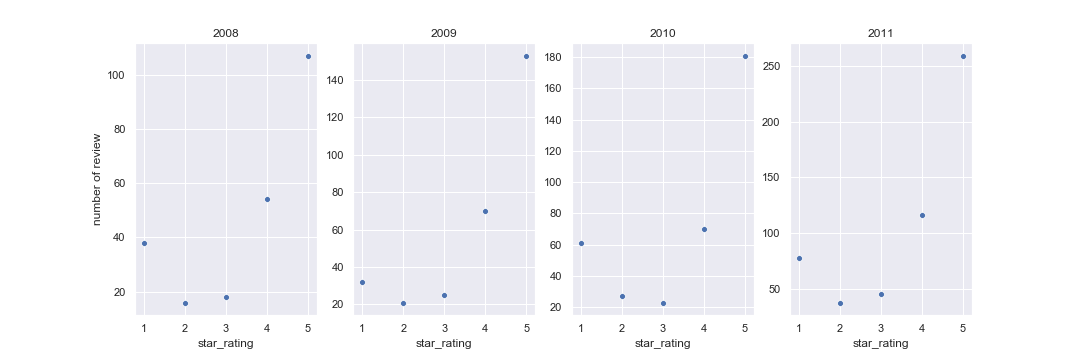
\includegraphics[width=10cm]{star_rating_to_number_of_review_2008-2011.png}
  \caption{Star rating to number of review 2008-2011} %\label{fig:lstm}
\end{figure}

\begin{figure}[!h]
  \small
  \centering
  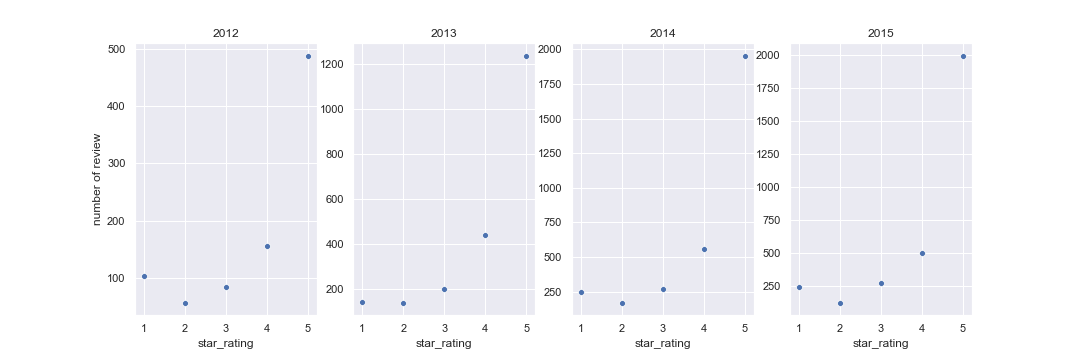
\includegraphics[width=10cm]{star_rating_to_number_of_review_2012-2015.png}
  \caption{Star rating to number of review 2012-2015} %\label{fig:lstm}
\end{figure}


In terms of the increment of the number of review, the influence of star number on the increment of comment number is increasing with the passing of time. Compared with low star rating, high star rating is more likely to bring the increment of comment number. At the same time, the distribution dispersion of comment number increment corresponding to low star rating is relatively small, while the variance of influence of high star rating on comment number increment is larger, which has higher uncertainty.

delta= Number of reviews in year n of a product - Number of reviews in year n-1 of a product
Mean star rating= The average star rating of a product in year n-1

After removing some abnormal points, from 2008 to 2012, the distribution of mean star rating on delta is symmetric with respect to the line delta =0. Therefore, we believe that mean star rating disturbs delta with an average value of 0. Between 2013 and 2014,there is a greater probability that a product with larger number of mean star rating will have larger increment of reviews. Available data for 2015 show that as of August 31, the increment in comments for the year was still marked with a delta=0 symmetry, possibly due to incomplete data.

\begin{figure}[!h]
  \small
  \centering
  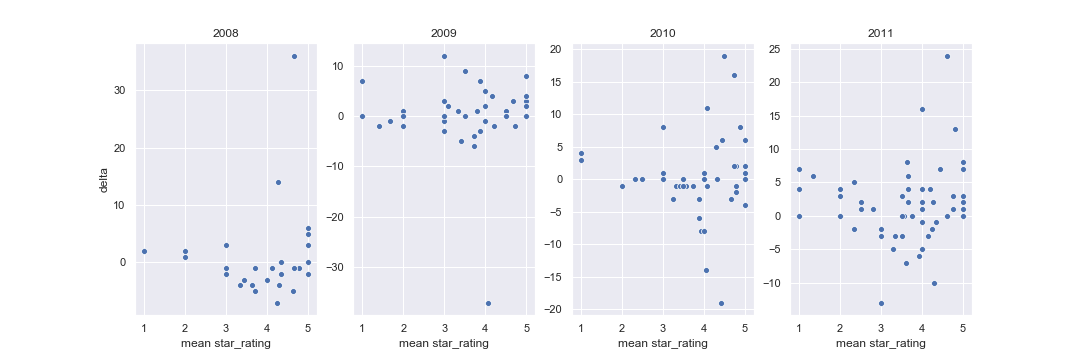
\includegraphics[width=10cm]{star_rating_to_delta_2008-2011.png}
  \caption{Star rating to delta 2008-2011} %\label{fig:lstm}
\end{figure}

\begin{figure}[!h]
  \small
  \centering
  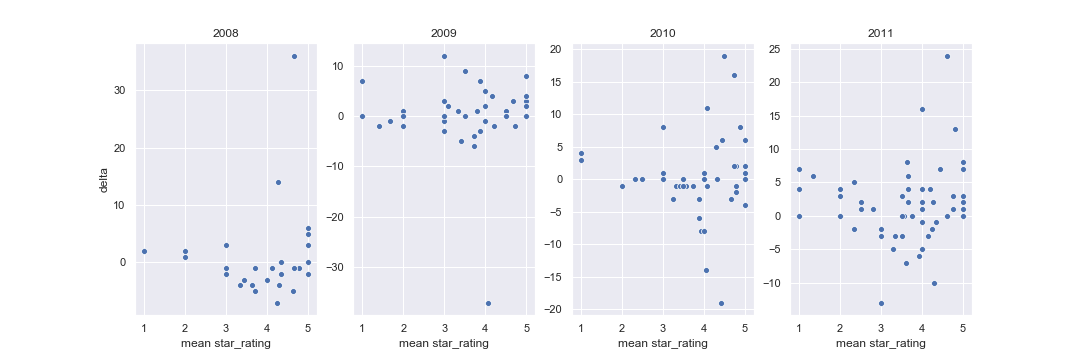
\includegraphics[width=10cm]{star_rating_to_delta_2008-2011.png}
  \caption{Star rating to delta 2008-2011} %\label{fig:lstm}
\end{figure}



\section{Conclusion}
  We use two models to do sentiment analysis: Naive Bayes Classifier and LSTM. There two models help us to select out some common featrues in postive and negative reviews, which is valuable for decision making. 

  To figure out how the reputation of product vary in a period of time, we construct the AHP-FCE model, through which we obtain a preliminary evaluation of products reputation.

  Also, we study the market factors by constructing the Multivariate Nonlinear Regression Model.

  In a nutshell, we find some valuable information for market descision making, which will be revealed in the memo.

  \section{Strength and Weakness}

  \subsection{Strength}
  
  \begin{enumerate}
  \item We used LSTM and naive bayesian models for emotion analysis respectively, and the results of these two methods were mutually verified with high accuracy.
  \item It has a strong theoretical and practical basis. The model we set is consistent with the real life situation of the change of commodity sales over time. The reputation we constructed is based on the reality and reflects the future trend of product sales. .And after parameter modification, the model can be applied to other markets.
  \item Universality..Our model can be widely applied to sentiment analysis of comment statements..
  \item Creativity。 We creatively simplifies the random factors in the time series model that we constructed, and from the result, this simplification process has little impact on results. In the future model construction, the random terms in the model can be replaced and the solving process of the model can be simplified on the premise of less influence on the results. 
  \end{enumerate}
  
  \subsection{Weakness} 
  \begin{enumerate}
  \item The parameters of the current model are only effective for the hair dryer market, and the other two markets need to find their own parameters.
  \item We use future comments as a metric, but this is not necessarily true. We lack convincing indicators to measure the potential sales of goods, and the existing reputation is only based on common sense and market theory.
  \item There is still some error in the best parameter we get, and maybe there is a better way to reduce it.
  \end{enumerate}




\newpage
\section{Memo}

\noindent From: MCM/ICM 2020 Team $\#$2020042

\noindent To: the Marketing Director of Sunshine Company

\noindent Date: March 10, 2020

\noindent Subject: Analysis and Suggestions on Online Marketing

From the data you provided, here we introduce our sentiment analysis model, AHP-FCE model and MNRM-MF(Multivariate nonlinear regression model based on market factors). Details and main results are as below:

\begin{itemize}
  \item Potentially important design features \\
   \begin{enumerate}
     \item hair dryer \\
     Most of the positive reviews mentioned “quiet”, ”powerful“, ”smooth” and “easy”, while most of the negative reviews focused on “dangerous”, “spark”, “fire”, “smell”. In conclusion, our design of hair dryer should be quiet, powerful, and easy to use. Safety is also a significant issue to pay attention to.
    \item Microwave \\
    “large”, “quickly”, “easy” are features praised most frequently in positive reviews, and some customers mentioned the power of the product. Meanwhile, many customers complain about their microwave using words “fix”, “repair”. To conclude, we should enhance the power of our microwave and make it easy to use. Also, our microwave ought to have a long service life.
    \item Pacifier \\
    "cute" is cited a lot in the positive reviews. Hence a pacifier which is cute and lovely may attract babies’ attention.
   \end{enumerate}
   \item Suggested online sales strategy: \\
    \begin{enumerate}
      \item We should speed up our express delivery. Products delivered quickly will earn more reputation.
      \item After-sale service should be paid attention to. Many customers made complaints about products’ after-sale service, which may have a negative impact on our reputation.
      \item We can employ online ghostwriters to improve the online “sentiment” of our products. Customers tend to write more reviews and give more feedbacks based on the contents of past reviews. 
      \item Company can take actions to promote their products during specific holidays, for example, Christmas Day.
    \end{enumerate}
\end{itemize}




\newpage

\begin{thebibliography}{99}
  \bibitem{1} S. Hochreiter, and J. Schmidhuber, “Long short-term memory,” Neural computation 9 (8): 1735--1780 (1997).
  \bibitem{2} Zijian Zheng and Geoffrey I. Webb . , “Lazy Learning of Bayesian Rules,”Machine Learning volume 41, pages53–84(2000)
  \bibitem{3} Freud, S., The Standard Edition of the Complete Works of Sigmund Freud, Vol. VII, J. Strachey (Ed.), London , Hogarth Press, 1958. 
  \bibitem{4} H. Zhang., N., “The Optimality of Naive Bayes”Psychother. Proceedings of the Seventeenth International Florida Artificial Intelligence Research Society Conference (FLAIRS 2004), AAAI Press, (2004)
  \bibitem{5} comScore/the Kelsey group, "Online Consumer-Generated Reviews Have Significant Impact on Offline Purchase Behavior" 2007.


  \end{thebibliography}




\end{document}

%% 
%% This work consists of these files mcmthesis.dtx,
%%                                   figures/ and
%%                                   code/,
%% and the derived files             mcmthesis.cls,
%%                                   mcmthesis-demo.tex,
%%                                   README,
%%                                   LICENSE,
%%                                   mcmthesis.pdf and
%%                                   mcmthesis-demo.pdf.
%%
%% End of file `mcmthesis-demo.tex'.
